\documentclass[12pt,a4paper]{article}
\usepackage[utf8]{inputenc}
\usepackage[italian]{babel}

\usepackage{rotating}
\usepackage{tabularx}
\usepackage{url}
\usepackage{float}
\usepackage{setspace}
\usepackage{parselines} 
\usepackage{graphicx}
\graphicspath{ {./img/} }

\usepackage{listings}
\usepackage{xcolor}



%New colors defined below
\definecolor{codegreen}{rgb}{0,0.6,0}
\definecolor{codegray}{rgb}{0.5,0.5,0.5}
\definecolor{codepurple}{rgb}{0.58,0,0.82}
\definecolor{backcolour}{rgb}{0.95,0.95,0.92}

%Code listing style named "mystyle"
\lstdefinestyle{mystyle}{
  backgroundcolor=\color{backcolour},   commentstyle=\color{codegreen},
  keywordstyle=\color{magenta},
  numberstyle=\tiny\color{codegray},
  stringstyle=\color{codepurple},
  basicstyle=\ttfamily\footnotesize,
  breakatwhitespace=false,         
  breaklines=true,                 
  captionpos=b,                    
  keepspaces=true,                 
  numbers=left,                    
  numbersep=5pt,                  
  showspaces=false,                
  showstringspaces=false,
  showtabs=false,                  
  tabsize=2
}

%"mystyle" code listing set
\lstset{style=mystyle}


\usepackage{geometry}
\usepackage{ragged2e}
\usepackage[svgnames]{xcolor}
\usepackage{makecell, tabularx}
    \setcellgapes{2pt}
    \makeatletter
    \newcommand*{\compress}{\@minipagetrue}
    \makeatother
    \newcolumntype{I}{ >{\RaggedRight\compress\itemize}X<{\enditemize}}
    \newcommand*{\mcl}[1]{\multicolumn{1}{l|}{#1}}
\usepackage[skip=1ex]{caption}
\usepackage{enumitem}





\usepackage{csquotes}


\title{Unità didattica sulla programmazione ad oggetti }
\author{Alessandro Freda}
\date{15-06-2020}

\usepackage{natbib}
\usepackage{graphicx}



\begin{document}

\maketitle


\section{Titolo}\label{titolo}
Principi dell’OOP: un percorso verso la progettazione di un videogioco... con Bob!

\section{Disciplina di riferimento}\label{disciplina-di-riferimento}

Informatica per un Liceo Scientifico indirizzo Scienze Applicate.

\section{Classe}\label{classe}

Questa UD è proposta per il quarto anno del Liceo Scientifico indirizzo Scienze Applicate. La classe è composta da 23 alunni. Nella classe si trovano grosse disparità tra gli studenti, alcuni eccellono altri, circa 6, sono poco attenti alle lezioni e non studiano costantemente. Il livello generale di conoscenza per la materia è medio, gli studenti fanno fatica a comprendere concetti più complessi e non riescono a risolvere esercizi più articolati in quanto non hanno buone fondamenta sulla programmazione.

\section{Motivazione e Finalità}\label{motivazione-e-finalituxe0}

Essendo la programmazione ad oggetti un argomento della programmazione abbastanza complessa per i novizi, in particolare per degli studenti di un liceo scientifico che hanno a disposizione poche ore settimanali per l’informatica, è necessario creare un’unità didattica volta a far comprendere al meglio questo argomento agli studenti con nuove metodologie didattiche attraverso la creazione di un videogioco.\\
Personalmente la programmazione ad oggetti è stata uno degli argomenti con cui ho avuto maggiori difficoltà nella comprensione durante il mio percorso di studi di informatica. Lo scopo di questa unità didattica è dunque quello introdurre i concetti base della programmazione ad oggetti cercando di coprire gli aspetti fondamentali dell’argomento partendo da metodologie che permettano allo studente la piena comprensione soprattutto mediante la creazione di schemi mentali corretti, è importante dunque che le lezioni siano coinvolgenti e che permettano allo studente di partecipare attivamente alla lezioni in modo da avere i maggiori risultati. 
 

\section{Prerequisiti}\label{prerequisiti}

Si presuppone che lo studente abbia familiarità con il linguaggio di programmazione Python.
I requisiti necessari per questa unità didattica sono:
\begin{itemize}
    \item Concetti base di programmazione
    \item Funzioni, definizione e chiamata
    \item Passaggio dei parametri 
\end{itemize}


\section{Contenuti}\label{contenuti}

Nella seguente unità didattica verranno insegnati i principi base della programmazione ad oggetti come richiesto dalle linee guida del ministero dell’istruzione per i licei scientifici ad indirizzo scienze applicate. 
Della programmazione ad oggetti verranno introdotti i seguenti argomenti: 
\begin{enumerate}
    \item Definizione di classe e definizione di istanza
    \item Costruttori e la parola chiave self
    \item Variabili di istanza e variabili di classe
    \item Metodi di istanza e metodi di classe
    \item Concetti di base dell'ereditarietà 
\end{enumerate}


\section{Obiettivi}\label{obiettivi}






\subsection{Collegamento con i documenti
ministeriali/proposte}\label{collegamento-con-i-documenti-ministerialiproposte}

La seguente unità didattica è volta ad insegnare l’argomento della programmazione ad oggetti seguendo le linee ministeriali presenti nel documento: \textit{“Indicazioni nazionali riguardanti gli obiettivi specifici di apprendimento concernenti le attività e gli insegnamenti compresi nei piani degli studi previsti per i percorsi liceali di cui all’articolo 10, comma 3, del decreto del Presidente della Repubblica 15 marzo 2010, n. 89, in relazione all’articolo 2, commi 1 e 3, del medesimo regolamento.”} Nelle seguenti linee guida ministeriali la programmazione ad oggetti è posta nel secondo biennio, dunque quarto anno, sotto l’area tematica di AL (algoritmi e linguaggi)



\subsection{Obiettivi}\label{obiettivi-1}

I seguenti obiettivi sono stati applicati sulla base della tassonomia qui presente (https://ibb.co/0ym4J8Z)

\begin{enumerate}
   \item Il conoscere
   \begin{itemize}
     \item Riprodurre la sintassi degli oggetti e delle classi in Python.
     \item Classificare oggetti di una stessa classe o oggetti di classi diverse. 
     \item Definire il concetto di istanza/oggetto. 
     \item Riconoscere un oggetto e la sua classe corrispondente.
     \item Riconoscere un problema risolvibile con la programmazione ad oggetti.
   \end{itemize}
   \item Il comprendere
   \begin{itemize}
     \item Descrivere la soluzione ad un problema mediante l'utilizzo della programmazione ad oggetti.
     \item Riconoscere un problema risolvibile con la programmazione ad oggetti.
     \item Applicare procedimenti volti all’utilizzo di classi ed oggetti.
     \item Verificare l’esecuzione del codice mediante un visualizer/tracer.
   \end{itemize}
   \item Pensiero convergente
   \begin{itemize}
     \item Analizzare un esercizio svolto mediante la programmazione ad oggetti.
     \item Schematizzare soluzioni per risolvere un problema con la programmazione ad oggetti.
   \end{itemize}
   \item pensiero divergente
   \begin{itemize}
     \item Formulare ipotesi di soluzione con oggetti che hanno come variabili altri oggetti.
     \item Riconoscere il problema dei modificatori di visibilità in una classe.
     \item Tentare soluzione con la programmazione ad oggetti per problemi risolvibili anche senza di essa.
   \end{itemize}
\end{enumerate}

\section{Metodologie didattiche}\label{metodologie-didattiche}


La seguente unità didattica è stata ideata sulla base di studi analizzati. La classe, per comprendere al meglio l’argomento della programmazione ad oggetti, sarà guidata attraverso un percorso che ricoprirà tutte le lezioni. Ogni lezione non sarà distinta dalle altre, ma saranno tutte collegate sulla base dello stesso principio: la creazione di un videogioco mediante la libreria PyGame \url{https://www.pygame.org/}. Gli studenti saranno invitati a creare gruppi nei quali applicheranno, con approcci di collaborative learning, i concetti esposti dal professore relativi al gioco. I componenti dei gruppi non saranno sempre gli stessi ma saranno scambiati più volte sulla base dell’andamento. Il docente esporrà esempi inerenti al videogioco e non esempi astratti. L’intento è quello di avvicinarsi ad una forma di costruzionismo che Papert definisce come “pensiero concreto” [1]. Mediante attività di "costruzione" (creazione di un videogioco) gli studenti saranno in grado di apprendere con maggiore efficacia. Si cerca di incentivare la fantasia degli studenti. \\
 Gli studi sulla didattica della programmazione ad oggetti analizzati [2] e [3], sostengo la tesi secondo cui coinvolgere gli studenti attraverso la creazione di giochi interattivi ed interessanti permette di mantenere la motivazione nello studio e allo stesso tempo consolidare i concetti studiati. Attraverso un approccio top-down il docente insegna passo dopo passo le principali funzioni della libreria e permetterà agli studenti di esprimersi liberamente con gli strumenti messi a disposizione. Uno dei problemi dell'insegnamento di un corso di programmazione è che gli studenti non sono ugualmente preparati. Risulta complesso personalizzare i contenuti del corso sulla base della preparazione personale degli studenti. Lo sviluppo di un gioco o esercizi in laboratorio permette agli studenti, anche quelli meno preparati, di divertirsi imparando. Gli studenti sono incoraggiati ad affrontare sfide sempre più impegnative. Pertanto, tutti gli studenti imparano e rendono significativo il progresso ottenuto durante lo svolgimento degli esercizi indipendentemente dalla loro preparazione. In classe dunque si svolgeranno solo attività relative allo sviluppo del videogioco, per casa possono invece essere assegnati esercizi generali sulla programmazione ad oggetti. In questo modo gli studenti oltre ad imparare a risolvere esercizi con difficoltà graduale saranno spinti ad applicare i concetti della programmazione ad oggetti in nuove forme creative mediante la creazione di un videogioco anche concepito sulle passioni personali.
\\L'obiettivo principale di questa unità didattica è, inoltre, quello di evitare che gli studenti creino misconcezioni sull’argomento ed essendo questa una didattica sulla programmazione, si cerca di favorire gli studenti a creare i giusti schemi mentali necessari per la comprensione e la concreta applicazione della programmazione ad oggetti. Si farà largo uso di strumenti di code visualizer per la visualizzazione della macchina concettuale \url{http://www.pythontutor.com/}.










\subsection{Il linguaggio che si adatta meglio alla didattica sulla programmazione ad oggetti}\label{scelta-linguaggio}
Prima della creazione della seguente unità didattica ho riflettuto a lungo su quale linguaggio di programmazione utilizzare. La scelta era tra Java e Python. La decisione non è stata semplice, Java è un linguaggio la cui caratteristica identitaria è la programmazione ad oggetti tuttavia è anche famoso per la difficoltà dovuta all’eccessiva sintassi che porta ad un maggiore carico cognitivo per gli studenti. Python, al contrario, risulta essere un linguaggio con un minor carico cognitivo, la cui sintassi è molto più snella ed ha la possibilità di utilizzare molti strumenti che facilitano la didattica e la comprensione degli argomenti agli studenti. Nonostante ciò anche Python (come Java) ha i suoi lati negativi, uno tra i quali è proprio la programmazione ad oggetti, la quale a mio parere non risulta comprensibile e inequivocabile quanto Java.\\Inoltre oggi nei licei molti professori avvicinano gli studenti al mondo della programmazione con Java e non con Python, una scelta che non è sempre condivisibile ma bisogna prenderne atto in quanto nella realtà ci si potrebbe ritrovare in una classe nella quale gli studenti hanno una maggiore padronanza del linguaggio Java e non Python. Ad un argomento complesso con un carico cognitivo notevole non si deve aggiungere il carico, già di per sé molto alto, del linguaggio di programmazione richiedendo agli studenti di impararne uno nuovo, seppur questo molto più semplice. Dunque è molto importante tenere conto del linguaggio di programmazione con il quale gli studenti hanno padronanza.\\La scelta per questa unità didattica, in conclusione, è ricaduta su Python. In questo caso Python permette di costruire lezioni coinvolgenti e allo stesso momento molto educative. Il carico cognitivo è nettamente inferiore, una sintassi più snella porterà gli studenti ad una maggiore comprensione dell’argomento. Infine anche la parte di debugging sarà molto più semplice. Un altro aspetto importante da considerare è il tempo a disposizione per la didattica, essendo in questo caso molto poco, Python è il linguaggio che meglio si adatta a questo tipo di situazione. Ho inoltre riassunto in una tabella quelle che, per me, sono i pro e i contro di Python e Java per l’insegnamento della programmazione ad oggetti. 



\begin{table}[H]
    \caption{Pro e contro dei linguaggi di programmazione Java e Python per la didattica sulla programmazione ad oggetti}
    \label{5.1}
    \makegapedcells
\setlist[itemize]{font=\color{DeepSkyBlue},
                  nosep,
                  leftmargin=*,
                  after=\vspace*{-\baselineskip}}
    \setlength{\tabcolsep}{3pt}
\begin{tabularx}{\linewidth}{|>{\RaggedRight}p{16mm}|*{2}{I |}}
    \hline

    &   \mcl{Pro}    &   \mcl{Contro}        \\
    \hline
Java
    &   \item Particolarmente adatto alla programmazione ad oggetti
        \item La chiarezza dei modificatori di accesso (o modificatori di visibilità) permette ai programmatori poco esperti di evitare di commettere errori di assegnazioni di variabili istanza o errori sui metodi istanza
        \item La presenza dell’operatore unario new usato per creare oggetti di una classe è molto utile per la fase di comprensione della creazione di un oggetto, essendo questo operatore utilizzato solo a questo scopo lo studente individua senza dubbi la fase di creazione di un oggetto
        \item Costruttori di una stessa classe con parametri diversi devono essere scritti separatamente (nella fase di comprensione è importante distinguere in maniera “visiva” il costruttore in base ai parametri)
        &   \item Eccessiva sintassi che porta ad un maggiore carico cognitivo durante la fase di comprensione della programmazione ad oggetti.
            \item Regole troppo restrittive, presenza quasi obbligatoria dei modificatori di accesso  e l’eccessiva sintassi porta lo studente a non concentrarsi sul concetto di programmazione ad oggetti e a distrarlo facilmente
            \item Necessita di più tempo a disposizione per la didattica
            \\
    \hline
Python
    &   \item Minore sintassi e minore carico cognitivo durante la fase di apprendimento 
        \item Maggiore libertà, non si richiedono modificatori di accesso
        \item Più semplice da leggere e da scrivere
        \item Sono disponibili molti tool per l’insegnamento 
        \item Nei casi in cui il tempo a disposizione per la didattica è poco Python è la migliore scelta 
        &   \item Regole non rigide non aiutano lo studente a comprendere al meglio i concetti portandolo spesso a commettere errori ed eventualmente creare misconcezioni
            \item Non esistono particolare restrizioni nell’accesso. Anche se un metodo è scritto con il doppio underscore come prefisso nel nome, il metodo non è mai realmente privato in quanto è facilmente accessibile utilizzando \_nomeclasse\_nomemetodoprivato
            \\
    \hline
\end{tabularx}
\end{table}




\section{Tempi}\label{tempi}
La seguente unità didattica è stata pensata per durare circa 3 mesi comprese le verifiche di apprendimento. Data la continuità delle lezioni, il numero può sensibilmente aumentare sulla base di vari fattori: l’andamento generale della classe, la comprensione dei concetti teorici, la svolgimento completo dei progetti. In un liceo scientifico scienze applicate il tempo messo a disposizione per la materia dell’informatica è di 2 ore alla settimana. Dato il grande spazio di tempo tra una lezione e l’altra verranno assegnati esercizi di consolidamento degli argomenti ad ogni fine lezione.
Ogni lezione ha la durata di 2 ore. Per questo argomento sono state ipotizzate:
\begin{itemize}
     \item 6 lezioni
     \item 1 verifica in itinere senza valutazione
     \item Eventuali lezioni di recupero/ripasso
     \item 1  verifica finale
   \end{itemize}



\section{Spazi}\label{spazi}


Tutte le lezioni sono composte da una parte teorica ed una pratica. Per questo motivo il laboratorio si rende necessario per tutte le lezioni. Per evitare che gli studenti si distraggano durante la lezione teorica, si ipotizza di svolgere queste parti in aula e durante la pausa spostarsi in laboratorio.\\
Per le lezioni teoriche è necessario un proiettore collegato ad un computer. Le lezioni che comprenderanno lo svolgimento dei progetti si svolgeranno in laboratorio. Nel caso in cui fosse possibile, gli studenti possono portare i proprio dispositivi ed utilizzarli in classe. Si incentiva inoltre l’utilizzo del raspberry [7], il quale integra perfettamente la libreria di Python PyGame che sarà utilizzata in tutte le lezioni. In questo caso è necessario avere a disposizione almeno 6/7 raspberry collegati a dei monitor in modo da creare gruppi da 3 nel quale gli studenti oltre a applicare la programmazione ad oggetti. Nel caso in cui non fosse possibile reperire dei raspberry l’esercizio finale può essere svolto in laboratorio con computer comuni.



\section{Materiali e Strumenti}\label{materiali}

\begin{itemize}
     \item Durante le lezioni saranno forniti agli studenti materiali prodotti dal docente (esercizi svolti, spiegazioni dettagliate e compiti da svolgere per la lezione successiva)
     \item Code visualizer online per la visualizzazione della macchina concettuale (\url{http://www.pythontutor.com/})
     \item Qualsiasi IDE per l’ambiente di sviluppo, se è possibile si incentiva l’utilizzo di Raspberry Pi
     \item Risorse online (wikipedia, esercizi svolti, documentazione Python e PyGame)
   \end{itemize}


\section{Percorso didattico}\label{percorso-didattico}



\subsection{Lezione 1} 

\subsection*{Prerequisiti}
Conoscenza della programmazione di base\\
Proiettore e computer\\
Ide e libreria PyGame


\subsection*{Finalità}
Gli studenti verranno introdotti al concetto della programmazione ad oggetti mediante una spiegazione teorica e pratica. Attraverso l’elaborazione della prima parte del videogioco gli studenti comprenderanno il concetto di classe e di istanza e saranno in grado di definire il concetto di istanza ed, inoltre, sapranno leggere il codice relativo alla programmazione ad oggetti in modo consapevole e critico. Si affronterà il concetto di istanza e variabile istanza al fine di far comprendere agli studenti la definizione di classe. 


\subsection*{Fasi dell'attività didattica: spazi e tempi}

\begin{enumerate}
	\item Introduzione sul lavoro da svolgere nella lezione e sul percorso della creazione del videogioco (20 minuti)
	\item Spiegazione teorica sui concetti base di classe ed istanza con esempi pratici basati sul videogioco (40 minuti)
	\item Discussione della classe sugli oggetti (15 minuti)
	\item Svolgimento in gruppi della prima parte del videogioco (40 minuti)
\end{enumerate}
La prima parte della lezione può essere svolta in classe, la seconda parte in laboratorio.

\subsection*{Cosa ho programmato di fare}
\begin{enumerate}
	\item Il docente fornisce il materiale ed espone alla classe gli argomenti dell’unità didattica e della lezione 1, mostrerà la libreria PyGame e il funzionamento del python tutor.
	\item Il docente introduce la programmazione ad oggetti mediante esempi concreti sul videogioco da creare nell’ora successiva. Nella spiegazione teorica si introducono i concetti base: creazione di una classe e definizione di istanza. Viene introdotto il concetto di costruttore. Vengono forniti esempi pratici sui concetti spiegati in precedenza, tali esempi potranno essere applicati nello svolgimento del videogioco. I concetti introdotti mediante il codice saranno visualizzati con l’utilizzo del code visualizer.
	\item Il docente invita gli studenti a fornire esempi di classi ed oggetti relativi ad un videogioco anche illustrando le idee alla lavagna, al fine di comprendere se ci sono misconcezioni ed eventualmente chiarire alcuni dubbi.
	\item Il docente chiede agli studenti di formare gruppi di massimo 3 persone e fornisce loro tutto il materiale utilizzato nella prima parte della lezione. Spiega agli studenti come consultare la libreria di PyGame e spiega loro come muovere i primi passi verso la prima parte del videogioco. 
\end{enumerate}
\subsection*{Cosa prevedo facciano gli alunni}

\begin{enumerate}
	\item Gli studenti raccolgono il materiale del professore ed ascoltano l’introduzione.
     \item Gli studenti ascoltano la spiegazione. In caso di dubbi chiedono chiarimenti e spiegazioni al docente.
\item Gli studenti forniscono esempi pratici di programmazione ad oggetti, anche mediante l’utilizzo della lavagna.
\item Gli studenti creano gruppi e cominciano a programmare, sulla base della spiegazione precedente e sul materiale fornito dal professore, il videogioco. Muovono i primi passi con PyGame ed applicano concretamente gli esempi, modificando gli oggetti e i nomi e creando il proprio videogioco. Leggono il codice fornito dal professore e cercano di interpretare il funzionamento del codice chiedendo al docente di spiegare con maggiore accuratezza le parti meno chiare.

\end{enumerate}

\subsection*{Materiali e strumenti}
Verranno forniti materiali inerenti alla lezione con relativo codice ed esempi, verranno forniti anche materiali supplementari online prodotti dal docente (video spiegazioni e esempi con codice)


\subsection*{Attività alternative / approfondimenti}
La lezione introduttiva può essere approfondita con svariati esempi sugli oggetti e sull’uso della programmazione ad oggetti nelle applicazioni, al fine di far comprendere agli studenti l’importanza e l’utilità dell’argomento.

\subsection*{Eventuali compiti a casa}
Sarà chiesto agli studenti di svolgere un esercizio composto da tre problemi da risolvere e da consegnare la settimana successiva. Gli studenti sono invitati a studiare il materiale prodotto dal docente ed integrare (non obbligatorio) il videogioco con nuove funzionalità.
\subsection*{In caso di studenti assenti}
Gli studenti assenti saranno invitati a studiare il materiale fornito dal professore ed a creare il proprio videogioco (la parte iniziale) a casa. In caso di dubbi potranno chiedere spiegazioni nella lezione successiva.













\subsection{Lezione 2} 

\subsection*{Prerequisiti}
Aver studiato il materiale fornito nella lezione 1 ed aver svolto la prima parte del videogioco\\
Proiettore e computer\\
Necessario un qualsiasi ide per python e un browser web per il code visualizer



\subsection*{Finalità}
Mediante l’elaborazione della seconda parte del videogioco gli studenti comprenderanno il concetto di creazione di diverse istanze di una stessa classe o di classi diverse. Si affronterà inoltre la parola chiave self, i costruttori e il concetto della visibilità delle variabili istanza e metodi istanza di una classe e l’accesso e modifica di quest’ultimi. La prima parte della lezione ha lo scopo di introdurre i concetti in modo teorico anche mediante l’utilizzo di codice ed esempi pratici relativi al videogioco. I concetti introdotti mediante il codice saranno visualizzati con l’utilizzo del code visualizer. Nella seconda parte della lezione gli studenti formeranno gruppi per l’elaborazione della seconda parte del videogioco, attraverso l’approccio del collaborative learning gli studenti, si confrontano tra di loro collaborando al fine di trasformare l’apprendimento in un processo attivo e coinvolgente [4]. Lo scopo del videogioco è, oltre a quello di suscitare l’interesse degli studenti, quello di evitare che gli studenti creino misconcezioni riguardo concetti della programmazione ad oggetti. Inoltre la collaborazione tra studenti crea anche competizione tra gruppi, creando uno spirito giocoso con la finalità di far partecipare attivamente tutti gli studenti della classe [3].


\subsection*{Fasi dell'attività didattica: spazi e tempi}

\begin{enumerate}
	\item Introduzione agli argomenti della lezione (15 minuti)
	\item Spiegazione teorica sul concetto di multiple istanze, parola self, costruttori, accesso e modifica di variabili e metodi istanza con esempi pratici basati sul videogioco (40 minuti)
	\item Svolgimento in gruppi della seconda parte del videogioco (40 minuti)
	\item Discussione sui progetti (20 minuti)
\end{enumerate}
La prima parte della lezione può essere svolta in classe, la seconda parte in laboratorio.

\subsection*{Cosa ho programmato di fare}
\begin{enumerate}
\item Il docente fornisce il materiale ed espone alla classe gli argomenti della lezione.
\item Il docente introduce i nuovi concetti attraverso una lezione teorica composta anche da esercizi svolti ed esempi pratici  su oggetti del videogioco.
\item Il docente invita gli studenti a ricomporre i gruppi ed iniziare ad applicare i concetti spiegati alla seconda parte del videogioco. Invita inoltre gli studenti ad implementare il proprio videogioco in maniera creativa utilizzando gli esempi forniti e avvalendosi dell’aiuto della documentazione di PyGame presente su internet.
\item Il docente chiede agli studenti di esporre le loro idee progettuali ed i principali problemi avuti e li aiuta a risolverli davanti alla classe.

\end{enumerate}
\subsection*{Cosa prevedo facciano gli alunni}

\begin{enumerate}
	\item Gli studenti raccolgono il materiale del professore.
	\item Gli studenti ascoltano la spiegazione. In caso di dubbi chiedono chiarimenti e spiegazioni al docente.
	\item Gli studenti in gruppi integrano il codice del proprio gioco sulla base della spiegazione fatta dal professore e sulla base del materiale fornito in precedenza.  Leggono il materiale cercano di interpretare il funzionamento del codice chiedendo al docente di spiegare con maggiore accuratezza le parti meno chiare. Implementano nuove funzionalità del videogioco con l’aiuto della documentazione di PyGame su internet.
	\item Gli studenti, un gruppo alla volta, espongono i principali problemi avuti e presentano le loro idee di implementazione. 


\end{enumerate}

\subsection*{Materiali e strumenti}

Verranno forniti materiali inerenti alla lezione con relativo codice ed esempi, verranno forniti anche materiali supplementari online prodotti dal docente (video spiegazioni e esempi con codice).


\subsection*{Attività alternative / approfondimenti}
Gli studenti sono invitati ad approfondire il progetto svolto in aula integrandolo a casa con nuove funzionalità (non obbligatorio). Nel materiale fornito dal docente saranno indicati siti sui quali gli studenti possono approfondire gli argomenti trattati nella lezione.  Sarà, inoltre, cura del docente fornire materiale autoprodotto al fine di fornire un maggior numero di esempi pratici e spiegazioni esaustive (anche mediante videolezioni).

\subsection*{Eventuali compiti a casa}
Per la lezione successiva sarà richiesto agli alunni di ripassare e studiare il materiale prodotto dal docente. Verranno assegnati esercizi da svolgere a casa e da consegnare al docente. 


\subsection*{In caso di studenti assenti}
Gli studenti assenti saranno invitati a studiare il materiale fornito dal professore e in caso di dubbi potranno chiedere spiegazioni nella lezione successiva. Potranno inoltre, riprendere il progetto ed aggiungere nuove funzionalità in linea con gli argomenti trattati nella seguente lezione.












\subsection{Lezione 3} 

\subsection*{Prerequisiti}
Aver studiato il materiale fornito nella lezione 2 ed aver svolto la seconda parte del videogioco\\
Proiettore e computer\\
Necessario un qualsiasi ide per python e un browser web per il code visualizer



\subsection*{Finalità}
La terza lezione ha lo scopo di consolidare gli argomenti trattati ed introdurre nuovi argomenti come la differenza tra variabili e metodi di istanza e variabili e metodi di classe. Verranno trattati gli argomenti sulle differenze tra variabili e metodi di istanza e di classe .La prima parte della lezione ha lo scopo di introdurre gli argomenti in modo teorico anche mediante l’utilizzo di codice ed esempi pratici relativi al videogioco. I concetti introdotti mediante il codice saranno visualizzati con l’utilizzo del code visualizer. Nella seconda parte della lezione gli studenti, in gruppi da 3, applicheranno i concetti introdotti dal professore nel videogioco integrando il lavoro fatto fino ad allora. 


\subsection*{Fasi dell'attività didattica: spazi e tempi}

\begin{enumerate}
    \item Introduzione alla lezione (15 minuti)
\item Spiegazione teorica sulle differenze tra variabili e metodi di istanza e di classe con esempi pratici basati sul videogioco (40 minuti)
\item Svolgimento in gruppi della terza parte del videogioco (40 minuti)
\item Discussione sui progetti (20 minuti)

\end{enumerate}
La prima parte della lezione può essere svolta in classe, la seconda parte in laboratorio.

\subsection*{Cosa ho programmato di fare}
\begin{enumerate}
\item Il docente fornisce il materiale ed espone alla classe gli argomenti della lezione.
\item Il docente introduce i nuovi concetti sulle differenze tra variabili e metodi di istanza e di classe attraverso una lezione teorica composta anche da esercizi svolti ed esempi pratici su oggetti del videogioco.
\item Il docente invita gli studenti a ricomporre i gruppi ed iniziare ad applicare i concetti spiegati alla terza parte del videogioco. Il docente può decidere di scambiare i componenti dei gruppi sulla base dell’andamento del progetto.
\item Il docente chiede agli studenti di esporre le loro idee progettuali ed i principali problemi avuti e li aiuta a risolverli davanti alla classe mostrando anche il codice svolto.

\end{enumerate}
\subsection*{Cosa prevedo facciano gli alunni}

\begin{enumerate}

\item Gli studenti raccolgono il materiale del professore ed ascoltano l’introduzione della lezione.
\item Gli studenti ascoltano la spiegazione. In caso di dubbi chiedono chiarimenti e spiegazioni al docente.
\item Gli studenti in gruppi integrano il codice del proprio gioco sulla base della spiegazione fatta dal professore e sulla base del materiale.
\item Gli studenti espongono i principali problemi avuti e presentano le loro idee di implementazione alla classe.

\end{enumerate}

\subsection*{Materiali e strumenti}
Verranno forniti materiali inerenti alla lezione con relativo codice ed esempi, verranno forniti anche materiali supplementari online prodotti dal docente (video spiegazioni ed esempi con codice).


\subsection*{Attività alternative / approfondimenti}
Gli studenti sono invitati ad approfondire il progetto svolto in aula integrandolo a casa con nuove funzionalità (non obbligatorio). Nel materiale fornito dal docente saranno indicati siti sui quali gli studenti possono approfondire gli argomenti trattati nella lezione.


\subsection*{Eventuali compiti a casa}
Per la lezione successiva sarà richiesto agli alunni di studiare il materiale fornito dal docente. Verranno assegnati 3 esercizi da svolgere a casa e da consegnare al docente per la lezione successiva. 


\subsection*{In caso di studenti assenti}
Gli studenti assenti saranno invitati a studiare il materiale fornito dal professore e in caso di dubbi potranno chiedere spiegazioni nella lezione successiva.  Potranno inoltre, riprendere il progetto ed aggiungere nuove funzionalità in linea con gli argomenti trattati nella seguente lezione.











\subsection{Lezione 4} 

\subsection*{Prerequisiti}
Aver studiato il materiale fornito nella lezione 3 ed aver svolto la terza parte del videogioco\\
Proiettore e computer\\
Necessario un qualsiasi ide per python e un browser web per il code visualizer



\subsection*{Finalità}
Nella quarta lezione gli studenti applicheranno mediante lo sviluppo del proprio videogioco il concetto di ereditarietà. Lo scopo di questa lezione è insegnare loro ad applicare l’ereditarietà a problemi la cui soluzione richiede questo argomento. La prima parte della lezione ha lo scopo di introdurre i concetti in modo teorico anche mediante l’utilizzo di codice ed esempi pratici relativi al videogioco. I concetti introdotti mediante il codice saranno visualizzati con l’utilizzo del code visualizer. Nella seconda parte della lezione gli studenti formeranno gruppi per l’elaborazione della quarta parte del videogioco, al fine di applicare concretamente il concetto di ereditarietà.


\subsection*{Fasi dell'attività didattica: spazi e tempi}

\begin{enumerate}
\item Introduzione sugli argomenti da trattare nella lezione e sulle modalità dello svolgimento della quarta parte del videogioco (15 minuti)
\item Spiegazione teorica sull’ereditarietà con esempi pratici basati sul videogioco (40 minuti)
\item Svolgimento quarta parte del videogioco (40 minuti)
\item Discussione sui progetti (20 minuti)

\end{enumerate}
La prima parte della lezione può essere svolta in classe, la seconda parte in laboratorio.

\subsection*{Cosa ho programmato di fare}
\begin{enumerate}
	\item Il docente fornisce il materiale ed espone alla classe gli argomenti della lezione.
\item Il docente introduce i nuovi concetti sull’ereditarietà attraverso una lezione teorica composta anche da esercizi svolti ed esempi pratici.
\item Il docente invita gli studenti a ricomporre i gruppi ed iniziare ad applicare i concetti spiegati alla quarta parte del videogioco.
\item Il docente chiede agli studenti di esporre le loro idee progettuali ed i principali problemi avuti e li aiuta a risolverli davanti alla classe.

\end{enumerate}
\subsection*{Cosa prevedo facciano gli alunni}

\begin{enumerate}
	\item Gli studenti raccolgono il materiale del professore.
\item Gli studenti ascoltano la spiegazione. In caso di dubbi chiedono chiarimenti e spiegazioni al docente.
\item Gli studenti in gruppi integrano il codice del proprio gioco sulla base della spiegazione fatta dal professore e sulla base del materiale, per aggiungere nuove funzionalità consultano la documentazione di PyGame e in caso di dubbi chiedono aiuto al docente e nei minuti finali espongono i problemi avuti alla classe.
\item Espongono le difficoltà avute durante lo svolgimento del videogioco e chiedono chiarimenti al professore mostrando il loro codice alla classe in modo che chiunque possa partecipare.

\end{enumerate}

\subsection*{Materiali e strumenti}
Verranno forniti materiali inerenti alla lezione con relativo codice ed esempi, verranno forniti anche materiali supplementari online prodotti dal docente (video spiegazioni ed esempi con codice).



\subsection*{Attività alternative / approfondimenti}
Gli studenti sono invitati ad approfondire il progetto svolto in aula integrandolo a casa con nuove funzionalità (non obbligatorio). Nel materiale fornito dal docente saranno indicati siti sui quali gli studenti possono approfondire gli argomenti trattati nella lezione. 

\subsection*{Eventuali compiti a casa}
Per la lezione successiva sarà richiesto agli alunni di studiare il materiale prodotto dal docente. Verranno assegnati 3 esercizi da svolgere a casa e da consegnare al docente per la lezione successiva.


\subsection*{In caso di studenti assenti}
Gli studenti assenti saranno invitati a studiare il materiale fornito dal professore e in caso di dubbi potranno chiedere spiegazioni nella lezione successiva. 














\subsection{Lezione 5} 

\subsection*{Prerequisiti}
Aver studiato il materiale fornito nella lezione 4 ed aver svolto la quarta parte del videogioco\\
Proiettore e computer\\
Necessario un qualsiasi ide per python e un browser web per il code visualizer 



\subsection*{Finalità}
La quinta ed ultima lezione prima della presentazione dei progetti ha lo scopo di introdurre gli argomenti dei metodi statici e del polimorfismo. Gli studenti concluderanno il progetto di gruppo e prepareranno la presentazione per la lezione successiva.


\subsection*{Fasi dell'attività didattica: spazi e tempi}

\begin{enumerate}
\item Introduzione agli argomenti della lezione odierna (15 minuti)
\item Spiegazione teorica sui metodi statici e sui concetti base del polimorfismo con esempi pratici basati sul videogioco (40 minuti)
\item Svolgimento parte finale del videogioco (1 ora)


\end{enumerate}
La prima parte della lezione può essere svolta in classe, la seconda parte in laboratorio.

\subsection*{Cosa ho programmato di fare}
\begin{enumerate}
	\item Il docente fornisce il materiale ed espone alla classe gli argomenti della lezione.
\item Il docente introduce i nuovi concetti sui metodi statici e sui concetti base del polimorfismo attraverso una lezione teorica composta anche da esercizi svolti ed esempi pratici sul videogioco "Il mondo di Bob".
\item Il docente invita gli studenti a ricomporre i gruppi ed iniziare ad applicare i concetti spiegati alla quarta parte del videogioco.


\end{enumerate}
\subsection*{Cosa prevedo facciano gli alunni}

\begin{enumerate}
\item Gli studenti raccolgono il materiale del professore. 
\item Gli studenti ascoltano la spiegazione. In caso di dubbi chiedono chiarimenti e spiegazioni al docente.
\item Gli studenti in gruppi integrano il codice del proprio gioco sulla base della spiegazione fatta dal professore e sulla base del materiale.


\end{enumerate}

\subsection*{Materiali e strumenti}

Verranno forniti materiali inerenti alla lezione con relativo codice ed esempi, verranno forniti anche materiali supplementari online prodotti dal docente (video spiegazioni ed esempi con codice).

\subsection*{Attività alternative / approfondimenti}

Gli studenti sono invitati ad approfondire il progetto svolto in aula integrandolo a casa con nuove funzionalità (non obbligatorio). Nel materiale fornito dal docente saranno indicati siti sui quali gli studenti possono approfondire gli argomenti trattati nella lezione. 

\subsection*{Eventuali compiti a casa}

Per la lezione successiva sarà richiesto agli alunni di creare slide riassuntive sul progetto svolto e di preparare una presentazione di gruppo. 

\subsection*{In caso di studenti assenti}
Gli studenti assenti saranno invitati a studiare il materiale fornito dal professore e in caso di dubbi potranno chiedere spiegazioni nella lezione successiva. Dovranno inoltre preparare la presentazione sul progetto svolto anche se incompleto.









\subsection{Lezione 6} 

\subsection*{Prerequisiti}
Lavagna e proiettore\\
Aver concluso il videogioco

\subsection*{Finalità}
Gli studenti attraverso l’esposizione del proprio videogioco si confrontano con la classe e con il professore. La presentazione davanti alla classe ha lo scopo di preparare gli studenti ad esporre, anche attraverso semplici slide, il lavoro svolto in modo da acquisire padronanza dell’argomento. Gli altri studenti che in quel momento non presentano possono intervenire proponendo una loro soluzione e allo stesso tempo confrontano, anche se indirettamente, il loro lavoro con quello degli altri.


\subsection*{Fasi dell'attività didattica: spazi e tempi}

\begin{enumerate}
	\item Esposizione videogiochi (2 ore)
\end{enumerate}
La lezione sarà interamente svolta in aula.

\subsection*{Cosa ho programmato di fare}
\begin{enumerate}
	\item Correggere alla classe gli eventuali errori e commentare le scelte progettuali. 
\end{enumerate}
\subsection*{Cosa prevedo facciano gli alunni}

\begin{enumerate}
	\item Ciascun gruppo espone il videogioco attraverso poche slide nelle quali riassume in punti ciò che è stato fatto, gli studenti sono invitati a partecipare e a fare commenti. In caso di dubbi gli studenti chiedono chiarimenti sia agli studenti che espongono sia al docente che risponde ai quesiti ed eventualmente corregge gli errori.
\end{enumerate}

\subsection*{Materiali e strumenti}
Per questa lezione non sono previsti materiali. Gli studenti presenteranno il videogioco attraverso slide sul computer della classe.
\subsection*{Attività alternative / approfondimenti}
Gli studenti sono invitati a modificare eventuali errori o ad aggiungere nuove features al videogioco.

\subsection*{Eventuali compiti a casa}
Non saranno assegnati nuovi compiti, gli studenti dovranno eventualmente modificare il codice sulla base di errori riscontrati nella presentazione dal professore o dalla classe. Gli studenti dovranno prepararsi per la verifica finale.










\section{Valutazione}\label{valutazione}

Gli studenti saranno valutati sulla base della loro capacità di esprimere, mediante esercizi pratici di programmazione e domande teoriche, di aver compreso i concetti base della programmazione ad oggetti. Essendo questo un argomento di programmazione non verranno effettuate interrogazioni orali, ma si valuterà il percorso dello studente anche attraverso l’esposizione orale finale del videogioco. La sufficienza si otterrà mostrando di aver compreso gli esercizi base dell’argomento. Progressivamente la valutazione migliorerà in base alla qualità sintattica del codice e alle soluzioni più efficienti.


\subsection{Valutazione in itinere /
formativa / per l'apprendimento}\label{valutazione-in-itinere-formativa}

Il docente terrà conto dei progressi dei singoli studenti sulla base del loro percorso durante le lezioni. Una verifica in itinere verrà svolta senza valutazione per permettere al docente di capire l’andamento della classe e correggere eventuali misconcezioni venutesi a creare in alcuni studenti. Mediante la verifica in itinere il docente sarà in grado di capire quali argomenti risultano più difficili e potrà modificare le lezioni sulla base degli errori degli studenti. La valutazione in itinere è dunque uno strumento molto importante per il docente anche per individuare gli studenti con maggiori difficoltà ed eventualmente concentrare parte delle lezioni a incentivare questi studenti ad esporre i problemi sorti durante lo svolgimento degli esercizi e dei progetti. 

\subsection{Valutazione sommativa / finale / dell'apprendimento}\label{valutazione-sommativa}

Si prevede una verifica finale con voto. Gli studenti potranno studiare dal materiale prodotto dal docente e dagli esercizi svolti durante il percorso e potranno anche consultare il libro di testo. La valutazione della verifica sarà composta da brevi esercizi da risolvere e domande teoriche. La valutazione finale terrà conto sia della verifica che del percorso dello studente. 
\clearpage
\section*{Bibliografia}

\begin{parse lines}[\noindent]{#1\\}


[1][Papert, S., 1986] \textit{Constructionism: A new opportunity for elementary science education}. NSF Grant Application.

[2][Yan, Lu. 2009] \textit{Teaching Object-Oriented Programming with Games.} ITNG 2009 - 6th International Conference on Information Technology: New Generations. 

[3][W. Chen and Y. C. Cheng 2007] \textit{"Teaching Object-Oriented Programming Laboratory With Computer Game Programming,"} in IEEE Transactions on Education, vol. 50, no. 3, pp. 197-203

[4][Yulia and R. Adipranata, 2010],  \textit{"Teaching object oriented programming course using cooperative learning method based on game design and visual object oriented environment,"}  2nd International Conference on Education Technology and Computer, Shanghai.

[5][Umberto Costantini, 2018] \textit{"Apprendimento della programmazione: analisi delle difficoltà e sviluppo di strategie didattiche"}. Tesi di laurea

[6][Lodi, 2014]\textit{ Imparare il pensiero computazionale, imparare a programmare.} Tesi di laurea, Università di Bologna, 2014.

[7][Davoli, 2014] \textit{ Solo Software Libero nella scuola!} 2014. \url{ http://aptiva.v2.cs.unibo.it/wiki/index.php/ Solo_Software_Libero_nella_scuola!}.






\end{parse lines}


\newpage
\appendix 
\section{Appendice: Materiali didattici per gli studenti}\label{appendice}
\subsection{(Lezione 1) Codice fornito dal professore per la realizzazione della prima parte del videogioco}

\begin{lstlisting}[language=Python, caption=Codice fornito dal professore per la realizzazione della prima parte del videogioco]

import pygame
import random
#grandezze espresse in pixel
LARGHEZZA = 800
ALTEZZA = 600
#Codici rgb
BIANCO = (255, 255, 255)
BLU = (0, 0, 255)
ROSSO = (255, 0, 0)

game_display = pygame.display.set_mode((LARGHEZZA,ALTEZZA))
pygame.display.set_caption('Il mondo di Bob')
clock = pygame.time.Clock()


class Giocatore:
    #Costruttore
    def __init__(self, nome, sesso):
        self.x = random.randrange(0, LARGHEZZA)
        self.y = random.randrange(0, ALTEZZA)
        self.nome = nome
        self.sesso = sesso

    #metodo per mostrare sullo schermo l'immagine dell'istanza
    def mostra(self, screen, immagine):
        screen.blit(immagine, (self.x, self.y))


class Ostacolo:
    #Costruttore
    def __init__(self, numero, pericolosità, movimento):
        self.x = random.randrange(0, LARGHEZZA)
        self.y = random.randrange(0, ALTEZZA)
        self.numero = numero
        self.pericolosità = pericolosità
        self.movimento = movimento


    #metodo per mostrare sullo schermo l'immagine dell'istanza
    def mostra(self, screen, immagine):
        screen.blit(immagine, (self.x, self.y))


    
def start():
    #creo istanza bob ed istanza ostacolo1 appartenenti
    #rispettivamente alle classi Giocatore ed Ostacolo
    bob = Giocatore('Bob', 'M')
    ostacolo1 = Ostacolo(1,5,False)

    #Carico le immagini da attribuire alle istanze
    bob_img = pygame.image.load('bob.png')
    ostacolo1_img = pygame.image.load('ostacolo1.png')
  

    while True:
        for event in pygame.event.get():
            if event.type == pygame.QUIT:
                pygame.quit()
                quit()
        #definisco lo sfondo del videogioco del colore bianco
        game_display.fill(BIANCO) 
        #mostro sullo schermo bob e l'ostacolo
        bob.mostra(game_display, bob_img)
        ostacolo1.mostra(game_display, ostacolo1_img)
        #richiamo il metodo muovi della classe Giocatore per muovere bob
        pygame.display.update()
        #definisco gli fps
        clock.tick(60)


start()
    


\end{lstlisting}

\newpage
\subsection{(Lezione 2) Materiale del professore}

Le classi, come abbiamo visto nella lezione precendente, permettono di includere variabili e funzioni in modo tale da essere riutilizzabili attraverso la creazione di istanze. Abbiamo creato la classe Giocatore con delle variabili istanza (x, y, nome, sesso) ed una classe Ostacolo con le variabili istanza (x, y, numero, pericolosità, movimento).


\begin{lstlisting}[language=Python, caption=Classe Giocatore]
class Giocatore:
    #Costruttore
    def __init__(self, nome, sesso):
        self.x = random.randrange(0, LARGHEZZA)
        self.y = random.randrange(0, ALTEZZA)
        self.nome = nome
        self.sesso = sesso
\end{lstlisting}

\begin{lstlisting}[language=Python, caption=Classe Ostacolo]
class Ostacolo:
    #Costruttore
    def __init__(self, numero, pericolosità, movimento):
        self.x = random.randrange(0, LARGHEZZA)
        self.y = random.randrange(0, ALTEZZA)
        self.numero = numero
        self.pericolosità = pericolosità
        self.movimento = movimento
\end{lstlisting}
\addvspace{20}
Abbiamo dunque creato l'istanza della classe Giocatore, denominandola Bob. Abbiamo poi creato l'istanza della classe Ostacolo, creando un vero e proprio ostacolo posizionato nel mondo di Bob.


\begin{lstlisting}[language=Python, caption=Istanze delle classi]
    #creo istanza bob ed istanza ostacolo1 appartenenti
    #rispettivamente alle classi Giocatore ed Ostacolo
    bob = Giocatore('Bob', 'M')
    ostacolo1 = Ostacolo(1,5,False)
\end{lstlisting}

\addvspace{20}
Applicandolo al videogioco con la libreria PyGame abbiamo mostrato graficamente le due istanze.

\begin{figure}[H]
\begin{center}
    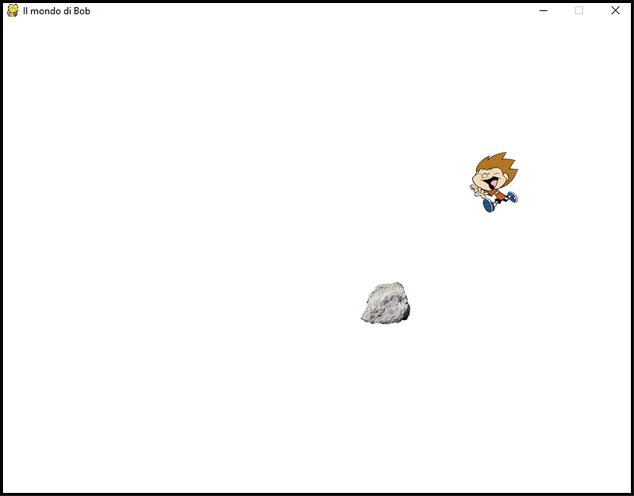
\includegraphics[width=\textwidth,height=\textheight,keepaspectratio]{img/1.png}
\end{center}
\caption{Videgioco il mondo di Bob}
\end{figure}



In questa lezione introduciamo alcuni concetti più avanzati sulle classi. Quando è stato introdotto il costruttore si è parlato della parola chiave self, vediamo nello specifico a cosa si riferisce. Nella lezione precedente si è affermato che all’interno di una classe non possono coesistere due variabili che hanno lo stesso nome, di conseguenza anche all’interno di un metodo non possono esserci due variabili dello stesso nome. Tuttavia se una di queste variabili è una variabile istanza questo è possibile. \\
La classe giocatore ha infatti le variabili istanza nome e sesso e queste sono precedute dalla parole chiave self (letteralmente “se stesso”) in quanto rappresenta l’oggetto che riceve l’invocazione del costruttore, mentre i parametri sono le variabili alle quali verranno associate le variabili istanza. Un costruttore è dunque un metodo che viene invocato quando viene creato un oggetto di una classe. Un costruttore fornisce il valore iniziale delle variabili di istanza dell’oggetto appena creato.\\
Essendo dunque una classe come uno stampo per la costruzione di oggetti (istanze) si possono creare multiple istanze di una stessa classe, vediamo un esempio. Nel mondo di Bob potremmo aggiungere un nuovo Player un amico ad esempio di nome Tom creando una nuova istanza della classe Giocatore in questo modo:


\begin{lstlisting}[language=Python, caption=Due istanze della classe Giocatore]
    bob = Giocatore('Bob', 'M')
    tom = Giocatore('Tome', 'M')
\end{lstlisting}
\addvspace{20}
Oppure è possibile creare molti ostacoli nel mondo di bob, creando una lista che li memorizza. Ad esempio possiamo creare una lista lista$\_$ostacoli che raggruppa tutti gli oggetti (istanze di tipo ostacolo):

\begin{lstlisting}[language=Python, caption=Multiple (20) istanze della classe ostacolo]
    lista_ostacoli = []
    for i in range(20):
        lista_ostacoli.append(Ostacolo(i,10,True))
\end{lstlisting}
\addvspace{20}
In questo modo possiamo mostrale sul videogioco per verificare la creazione delle diverse istanze, 
Mostrando graficamente le istanze possiamo notare le 20 istanze della classe ostacolo nel mondo di Bob:

\begin{figure}[H]
\begin{center}
    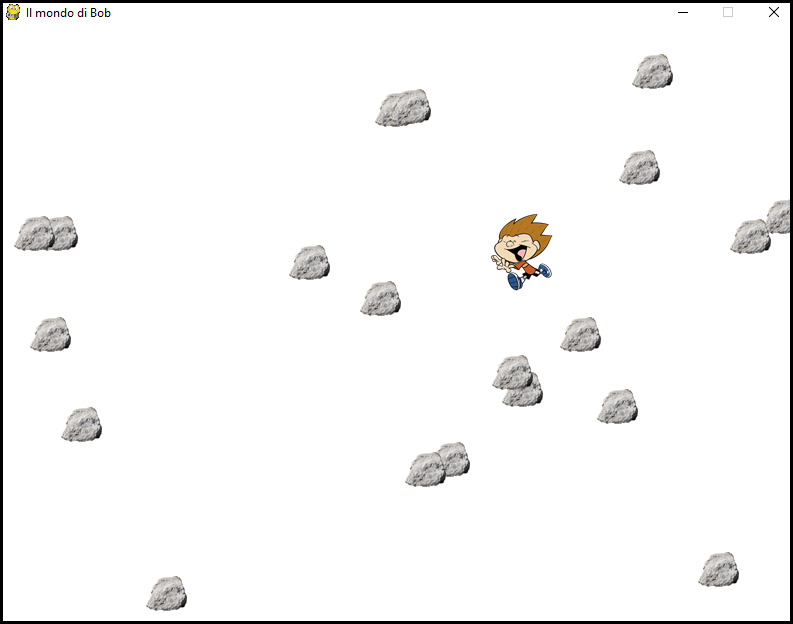
\includegraphics[width=\textwidth,height=\textheight,keepaspectratio]{img/bob_multiple_istanze.PNG}
\end{center}
\caption{Multiple (20) istanze della classe ostacolo mostrate graficamente}
\end{figure}

Come introdotto nella prima lezione un metodo è un insieme di istruzioni con un nome la cui invocazione comporta l’esecuzione delle istruzioni in esso definite. Un metodo istanza è un metodo che viene invocato su un oggetto è che può manipolare lo stato dell’oggetto stesso.Un metodo di istanza definito in una classe viene invocato usando un oggetto di quella classe. L'oggetto prende il nome di oggetto chiamante (calling object). L’invocazione viene effettuata scrivendo il nome dell’oggetto, per esempio bob, seguito da un punto e dal nome del metodo, per esempio bob.muovi() ed infine da una coppia di parentesi che possono contenere i parametri per il metodo. Tutte le definizioni di metodo istanza compaioni della definizione della classe alla quale appartengono. Questi metodi infatti possono essere usati solo con oggetti della classe in cui il metodo è definito.  

\begin{lstlisting}[language=Python, caption=Metodo istanza muovi() della classe Giocatore]
def muovi(self):
        #nella variabile key_input memorizza il pulsante premuto
        key_input = pygame.key.get_pressed()  
        #sposta l'istanza di 5 pixel
        if key_input[pygame.K_LEFT]:
            self.x -= 5
        if key_input[pygame.K_UP]:
            self.y -= 5
        if key_input[pygame.K_RIGHT]:
            self.x += 5
        if key_input[pygame.K_DOWN]:
            self.y += 5
\end{lstlisting}
\addvspace{20}
Allo stesso modo possiamo mettere in movimento anche gli oggetti ostacolo, defininendo un movimento random.

\begin{lstlisting}[language=Python, caption=Metodo istanza muovi() della classe Ostacolo]
def muovi(self):
        if self.movimento:
            self.x += random.randrange(-4,5)
            self.y += random.randrange(-4,5)

            #controllo per evitare che si muovano oltre i bordi
            if self.x < 0: self.x = 0
            elif self.x > LARGHEZZA: self.x = LARGHEZZA
        
            if self.y < 0: self.y = 0
            elif self.y > ALTEZZA: self.y = ALTEZZA
        else:
            print("L'ostacolo non si può muovere")
\end{lstlisting}
\addvspace{20}

Vediamo ora come accedere ai valori delle variabili istanza di un oggetto. Abbiamo visto come un oggetto di una classe è un elemento contenente al proprio interno una serie di variabili di istanza. Le variabili istanze in python sono accessibili e modibicabili anche esternamente alla definizione della classe. Bisogna porre dunque molta attenzione quando si modifica o accede ad una variabile di una istanza in quanto è possibile modificarla in modo molto semplici attraverso la sintassi nomeoggetto.variabileIstanza. \\
Facciamo un esempio pratico, preso il nostro esempio di Bob vogliamo mostrare a video la posizione di Bob durante lo spostamento. Quello che dobbiamo fare è prendere i valori delle coordinate x ed y dell'istanza Bob e mostrarla a video. Per fare ciò creaiamo due variabili posizioneBob$\_$x e posizioneBob$\_$y nelle quali memorizziamo le posizioni delle coordinate x ed y di bob. 

\begin{lstlisting}[language=Python, caption=Accesso al valore delle variabili istanza]
        posizioneBob_x = bob.x
        posizioneBob_y = bob.y
\end{lstlisting}
\addvspace{20}

Possiamo ora mostrare in tempo reale le coordinate di bob nella mappa stampando i valori delle variabili memorizzate: 

\begin{lstlisting}[language=Python, caption=Codice per mostrare sulla mappa le coordinate di Bob]
        #mostro sulla schermo le coordinate di Bob
        textsurface = myfont.render(f'Bob si trova nelle coordinate: x: {str(posizioneBob_x)} y: {str(posizioneBob_y)}',False, (0, 0, 0))
        game_display.blit(textsurface,(450,550))
\end{lstlisting}
\addvspace{20}

Vediamo ora il risultato finale:

\begin{figure}[H]
\begin{center}
    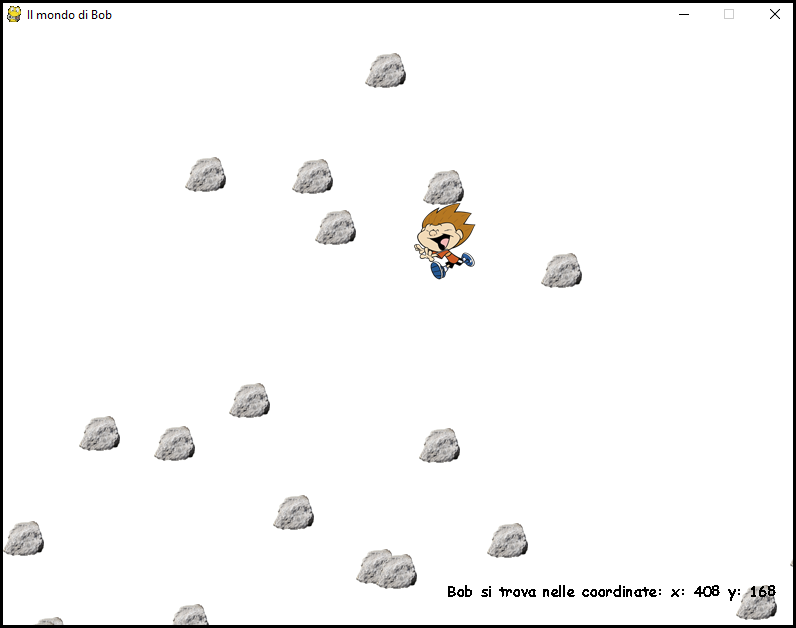
\includegraphics[width=\textwidth,height=\textheight,keepaspectratio]{img/coordinate.PNG}
\end{center}
\caption{Coordinate di bob mostrate graficamente in modo dinamico}
\end{figure}

Nella lezione di oggi abbiamo visto nello specifico il concetto di classe che possiede delle variabili istanza per memorizzare dati e definizioni di metodi che eseguono azioni. Abbiamo poi visto cosa è un costruttore, ovvero un metodo che, invocato, crea ed inizializza un oggetto di una classe. Le variabili istanza e i metodi istanza possono essere usati da qualunque posizione. Abbiamo poi visto nello specifico la parola chiave self , la quale quando è usata all'interno della definizione di classe rappresenta l'oggetto che riceve l'invocazione di un metodo. Sulla base di questi concetti teorici abbiamo poi creato un videogioco interattivo composto da un giocatore Bob (istanza della classe Giocatore) ed una serie di ostacoli (20 istanze della classe Ostacolo) che si muovono nel mondo di Bob ed ostacolano il suo movimento nello spazi. Nelle prossime lezione parleremo di variabili di classe, le quali a differenza delle variabili istanza sono attributi che vengono condivisi da tutte le Istanze della Classe. Parleremo poi dei metodi di classe, metodi che permettono di passare come parametro la Classe invece dell'Istanza.

\addvspace{20}
Riassunto in punti dei concetti trattati nella lezione di oggi:
\begin{itemize}
     \item Le classi hanno variabili di istanza per memorizzare dati e definizioni di metodi che eseguono azioni.
     \item Un costruttore è un metodo che, invocato, crea ed inizializza un oggetto di una classe.
     \item Si possono creare diverse istanze di una stessa classe, con parametri uguali o diversi.
     \item La parola self, quando usata all'interno di una definizione di un metodo (incluso il costruttore), rappresenta l'oggetto che riceve l'invocazione di metodo.
     \item Le variabili istanza e i metodi istanza possono essere usati (modifica ed accesso) da qualunque posizione.
   \end{itemize}
\addvspace{20}  
Di seguito il codice completo del videogioco creato fino ad ora:

\begin{lstlisting}[language=Python, caption=Codice videogioco "Il mondo di Bob" della seconda lezione]
import pygame
import random

#grandezze espresse in pixel
LARGHEZZA = 800
ALTEZZA = 600
#Codici rgb
BIANCO = (255, 255, 255)
BLU = (0, 0, 255)
ROSSO = (255, 0, 0)
#impostazioni di gioco (schermo e clock)
game_display = pygame.display.set_mode((LARGHEZZA,ALTEZZA))
pygame.display.set_caption('Il mondo di Bob')
clock = pygame.time.Clock()
class Giocatore:
    #Costruttore
    def __init__(self, nome, sesso):
        self.x = random.randrange(0, LARGHEZZA)
        self.y = random.randrange(0, ALTEZZA)
        self.nome = nome
        self.sesso = sesso


    def muovi(self):
        #nella variabile key_input memorizza il pulsante premuto
        key_input = pygame.key.get_pressed()  
        #sposta l'istanza di 5 pixel
        if key_input[pygame.K_LEFT]:
            self.x -= 5
        if key_input[pygame.K_UP]:
            self.y -= 5
        if key_input[pygame.K_RIGHT]:
            self.x += 5
        if key_input[pygame.K_DOWN]:
            self.y += 5

    #metodo per mostrare sullo schermo l'immagine dell'istanza
    def mostra(self, screen, immagine):
        screen.blit(immagine, (self.x, self.y))

class Ostacolo:
    #Costruttore
    def __init__(self, numero, pericolosità, movimento):
        self.x = random.randrange(0, LARGHEZZA)
        self.y = random.randrange(0, ALTEZZA)
        self.numero = numero
        self.pericolosità = pericolosità
        self.movimento = movimento
    
    def muovi(self):
        if self.movimento:
            #movimento random da -4 a 4 pixel
            self.x += random.randrange(-4,5)
            self.y += random.randrange(-4,5)

            #controllo per evitare che si muovano oltre i bordi
            if self.x < 0: self.x = 0
            elif self.x > LARGHEZZA: self.x = LARGHEZZA
        
            if self.y < 0: self.y = 0
            elif self.y > ALTEZZA: self.y = ALTEZZA
        else:
            print("L'ostacolo non si può muovere")
    
    #metodo per mostrare sullo schermo l'immagine dell'istanza
    def mostra(self, screen, immagine):
        screen.blit(immagine, (self.x, self.y))


    
def start():
    #creo istanza bob ed istanze ostacolo appartenenti
    #rispettivamente alle classi Giocatore ed Ostacolo
    bob = Giocatore('Bob', 'M')
    lista_ostacoli = []
    for i in range(20):
        lista_ostacoli.append(Ostacolo(i,10,True))

    #Carico le immagini da attribuire alle istanze
    bob_img = pygame.image.load('bob.png')
    ostacolo1_img = pygame.image.load('ostacolo1.png')
    #definisco il font per il testo 
    pygame.font.init() 
    myfont = pygame.font.SysFont('Comic Sans MS', 15, True)
    

    while True:
        for event in pygame.event.get():
            if event.type == pygame.QUIT:
                pygame.quit()
                quit()
        #definisco lo sfondo del videogioco del colore bianco
        game_display.fill(BIANCO) 
        #mostro sullo schermo bob e l'ostacolo
        bob.mostra(game_display, bob_img)
        #mostro sulla mappa tutti gli ostacoli e li metto in movimento
        for i in lista_ostacoli:
            i.mostra(game_display, ostacolo1_img)
            i.muovi()
        #richiamo il metodo muovi della classe Giocatore per muovere bob
        bob.muovi()
        #variabili che memorizzano le coordinate di bob
        posizioneBob_x = bob.x
        posizioneBob_y = bob.y
        #mostro sulla schermo le coordinate di Bob
        textsurface = myfont.render(f'Bob si trova nelle coordinate: x: {str(posizioneBob_x)} y: {str(posizioneBob_y)}',False, (0, 0, 0))
        #posiziono e mostro il testo nella mappa
        game_display.blit(textsurface,(450,550))
        pygame.display.flip()
        pygame.display.update()
        #definisco gli fps
        clock.tick(60)
        
start()

\end{lstlisting}
\addvspace{20}






\newpage

\section{Licenza del documento}\label{licenza}

Quest'opera è stata rilasciata con licenza Creative Commons Attribuzione - Condividi allo stesso modo 4.0 Internazionale. Per leggere una copia della licenza visita il sito web \url{http://creativecommons.org/licenses/by-sa/4.0/} o spedisci una lettera a Creative Commons, PO Box 1866, Mountain View, CA 94042, USA.


\end{document}
